\section{Gustavo A. Medrano-Cerda - Comparison of Various Active Impedance Control Approaches, Modeling, Implementation, Passivity, Stability and Trade-offs - 2012}
\subsection*{Summary}
Four main controllers have been here compared, all of them have in common the outer control loop based on torque feedback. These controllers are targeted at SEA (Series Elastic Actuators) where each motor is coupled with a elastic and damping factor. The Impedance control (IC) is achieved with a torque feedback:\\ "on motor side": $ \tau_d = \tau_c + K (\theta_{ref}-\theta_{mH}) - D(\dot{\theta}_{mH})$\\ or on the "link side: $ \tau_d = \tau_c + K (\theta_{ref}-\theta_{L}) - D(\dot{\theta}_{L})$\\
IC control can either be based on \textbf{motor side} or \textbf{link side}, thus all of the controllers shown below can have two possible versions. The motor side consists in supplying as a feedback the motor angles $\theta_m$ while the link side consists in supplying the link states $\theta_L$. These two states might differ mainly because of the elasticity of the links. The following controllers differ from the inner loop and the type of reference signal that the outer IC loop provides to the inner controller:
\begin{itemize}
\item ICT = Impedance control with explicit torque loop (and inner torque PID loop)
\item ICP = IC torque control with inner position PID control (damping gain D as small as possible)
\item ICVM = outer torque loop and inner velocity PI gain (motor side). This method could be used on HyQ (note that the term $\frac{1}{D}$ requires the damping gain D to be always quite big, which is the case for HyQ). The advantage of using the inner velocity-based PI controller is that passivity is granted also for high values of systems stiffness (which is not true for the torque-based PID);
\item ICVL = outer torque loop and inner velocity PI gain (link side);
\end{itemize}
\subsection*{Take aways}
\begin{itemize}
\item In the design of nested control loops it's not always sufficient to design the inner loop (of whichever kind, e.g. PID) with the highest bandwidth possible (chiefly when we deal with discrete systems). It was here shown that the outer \textbf{impedance control} loop (on \textbf{motor or link side}) might not be stable even for very high bandwidth of the inner loop. 
\item It is sometimes interesting to check the bandwidth not only of the overall controller but also of the innermost PID loop. The table below (figure \ref{ICperformance}) provides some performance of the bandwidth for different impedance controllers (ICT, ICP and ICV).\begin{figure}[h!]
  \centering
  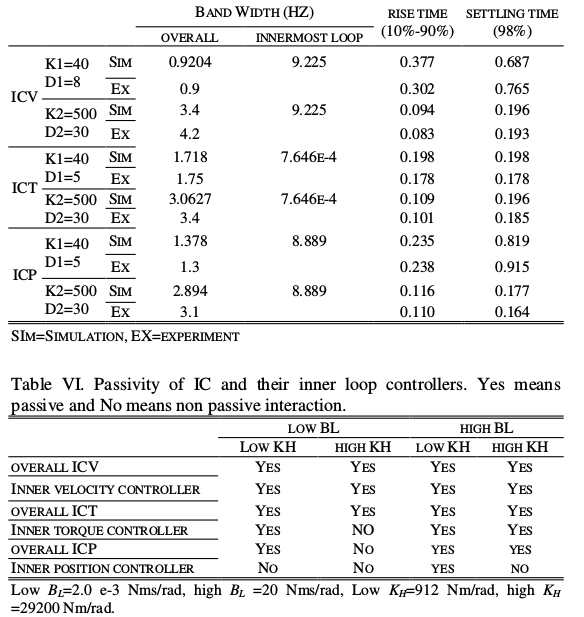
\includegraphics[width=120mm]{PassivityOfICcontrollers}
  \caption{Performance of ICT, ICP and ICV with respect to passivity for low and high stiffness and damping gains}
  \label{ICperformance}
\end{figure}
The bandwidth of the innermost PID loop is of importance when we have the inner PID loop running on the DSP (Digital Signal Processing) unit and we have the outer loop (impedance control) running on a centralized CPU. In the case the communication fails then the actuator will be left with the inner PID loop only. For this reason the higher the bandwidth of the inner loop the more robust is the system again communication failures.
\end{itemize}
